\providecommand{\graphTheoryPreambleLoaded}{}
\ifx\graphTheoryPreambleLoaded
\documentclass{article}
\usepackage{./1_Preamble/graph_theory_preamble}

\begin{document}
	\fi
	
	\newpage
	\subsection*{Shortest Route}
	\addcontentsline{toc}{subsection}{Shortest Route}
	A shortest route can be defined as \textit{searching for the least weights within a graph}.
	From the perspective of this game, this is essentially useful for traveling from any initial arbitrary point to the desired ending point fast. \\
	
	This can be helpful for players that just wants to finish the mission early by employing such methods. Speedrunners who wants to finish the game as fast as they can. Which they apply some of the known shortest path algorithms such as \textbf{Dijkstra} or \textbf{A*} with respect on how they implement their optimized node placement in order to get the optimal time to complete all missions. \\
	
	Due to how valuable this concept is to videogames, almost all open-world games today implement waypoints for the player to take advantage of. Starting from Grand Theft Auto: IV, up to the new  and upcoming Grand Theft Auto: VI, the waypoint system has evolved to use increasingly refined path-finding algorithms to guide players through its environments. \\
	
	Unfortunately, this was not yet implemented in Grand Theft Auto: San Andreas, which is also fortunate enough that we can implement and experiment with our own shortest path route to enhance the gameplay experience.
	
	\subsubsection*{Dijkstra's Algorithm}
	\addcontentsline{toc}{subsubsection}{Dijkstra's Algorithm}
	For finding the shortest path within the graph, we shall utilize the most popular shortest route algorithm, the Dijkstra's Algorithm.
	\begin{algorithm}[Dijkstra's Algorithm]
		The algorithmic procedure for the Dijkstra's Algorithm states that
		\begin{enumerate}
			\item[Step 1] \textbf{Initialize} the distances of every vertices \(\text{dist}(V(G))\) to have \textbf{infinite \(\infty\) distance}.
			\item[Step 2] Start with the current source vertex \(v_{1}\) with distance \(d_{ij} = 0\).
			\item[Step 3] For every adjacent vertices \(v_{i}\) of \(v_{1}\), mark them as a \textbf{potential shortest distance}.
			\item[Step 4] The shortest distance of the adjacent vertices from \(v_{1}\) will now be the \textbf{successor} of that source vertex. Let us call it \(v_{j}\).
			\item[Step 5] Mark \(v_{1}\) to be a \textbf{visited} vertex, and move on to \(v_{j}\).
			\item[Step 6] \textbf{Repeat} the process until all vertices are \textbf{visited} and we have found the optimal value \(d_{ij}\) to get to the sink vertex \(v_{f}\).
		\end{enumerate} This algorithm will produce a \textbf{time complexity} of \(O((n + m)\cdot log(n))\), where \(n\) is the order and \(m\) is the size of graph \(G\).
	\end{algorithm} We shall use the following table as a guide in how we will implement the algorithm into our chosen graph.
	\begin{longtable}[c]{@{}ccc|l@{}}
		\toprule
		Vertex & \begin{tabular}[c]{@{}c@{}}Shortest \\ Distance\end{tabular} & \begin{tabular}[c]{@{}c@{}}Previous \\ Vertex\end{tabular} & Optimal Value = 0.00  \\* \midrule
		\endfirsthead
		%
		\multicolumn{4}{c}%
		{{\bfseries Table \thetable\ continued from previous page}} \\
		\endhead
		%
		\bottomrule
		\endfoot
		%
		\endlastfoot
		%
		\(v_1\) & 0    & \(v_1\) & Visited = \{\(\varnothing\)\}                         \\
		\(v_2\) & \(\infty\)  & NA   & Unvisited = \(\{v_1, v_2, \dots, v_k\}\) \\
		\(\vdots\) & \(\vdots\) & \(\vdots\) &                   \\
		\(v_k\) & \(\infty\)  & NA   &                                        \\* \bottomrule
		\caption{Shortest Path Table}
		\label{route_table}\\
	\end{longtable}
	
	\subsubsection*{Implementation}
	\addcontentsline{toc}{subsubsection}{Implementation}
	Since \(|V(G)|~\text{and}~|E(G)|\) are enormous, we will not go over the step-by-step procedure as to how we developed its shortest path. Instead, we shall look over the graph with its shortest path. Then analyze where we should go in-game in order to get to the desired location. Followed with how we employ the algorithm using the table similar to table (\ref{shortest_route}) \newpage
	\begin{figure}[!h]
		\centering
		\begin{minipage}{0.49\textwidth}
			\centering
			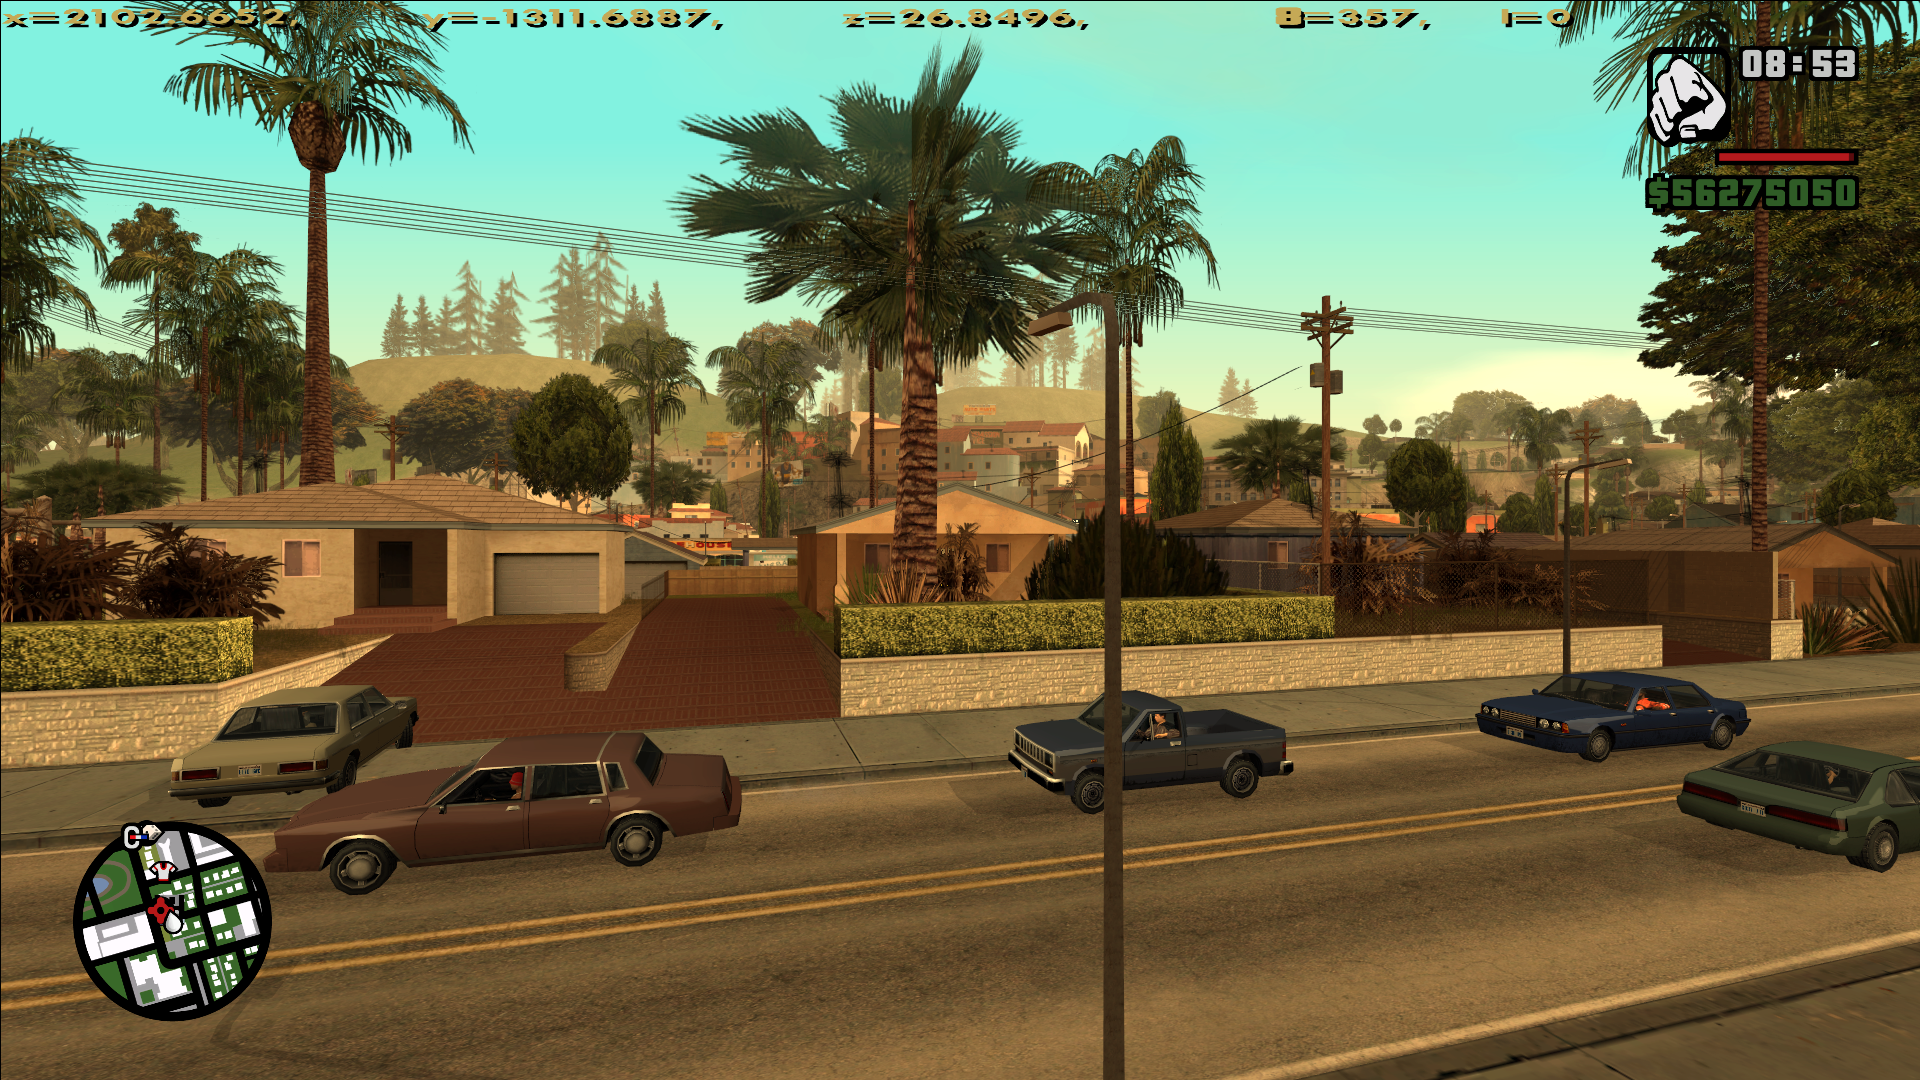
\includegraphics[width=1\textwidth]{./0img/sourceVertex.png}
			\subcaption{Initial Location \(S\)}
		\end{minipage}
		\hfill
		\begin{minipage}{0.49\textwidth}
			\centering
			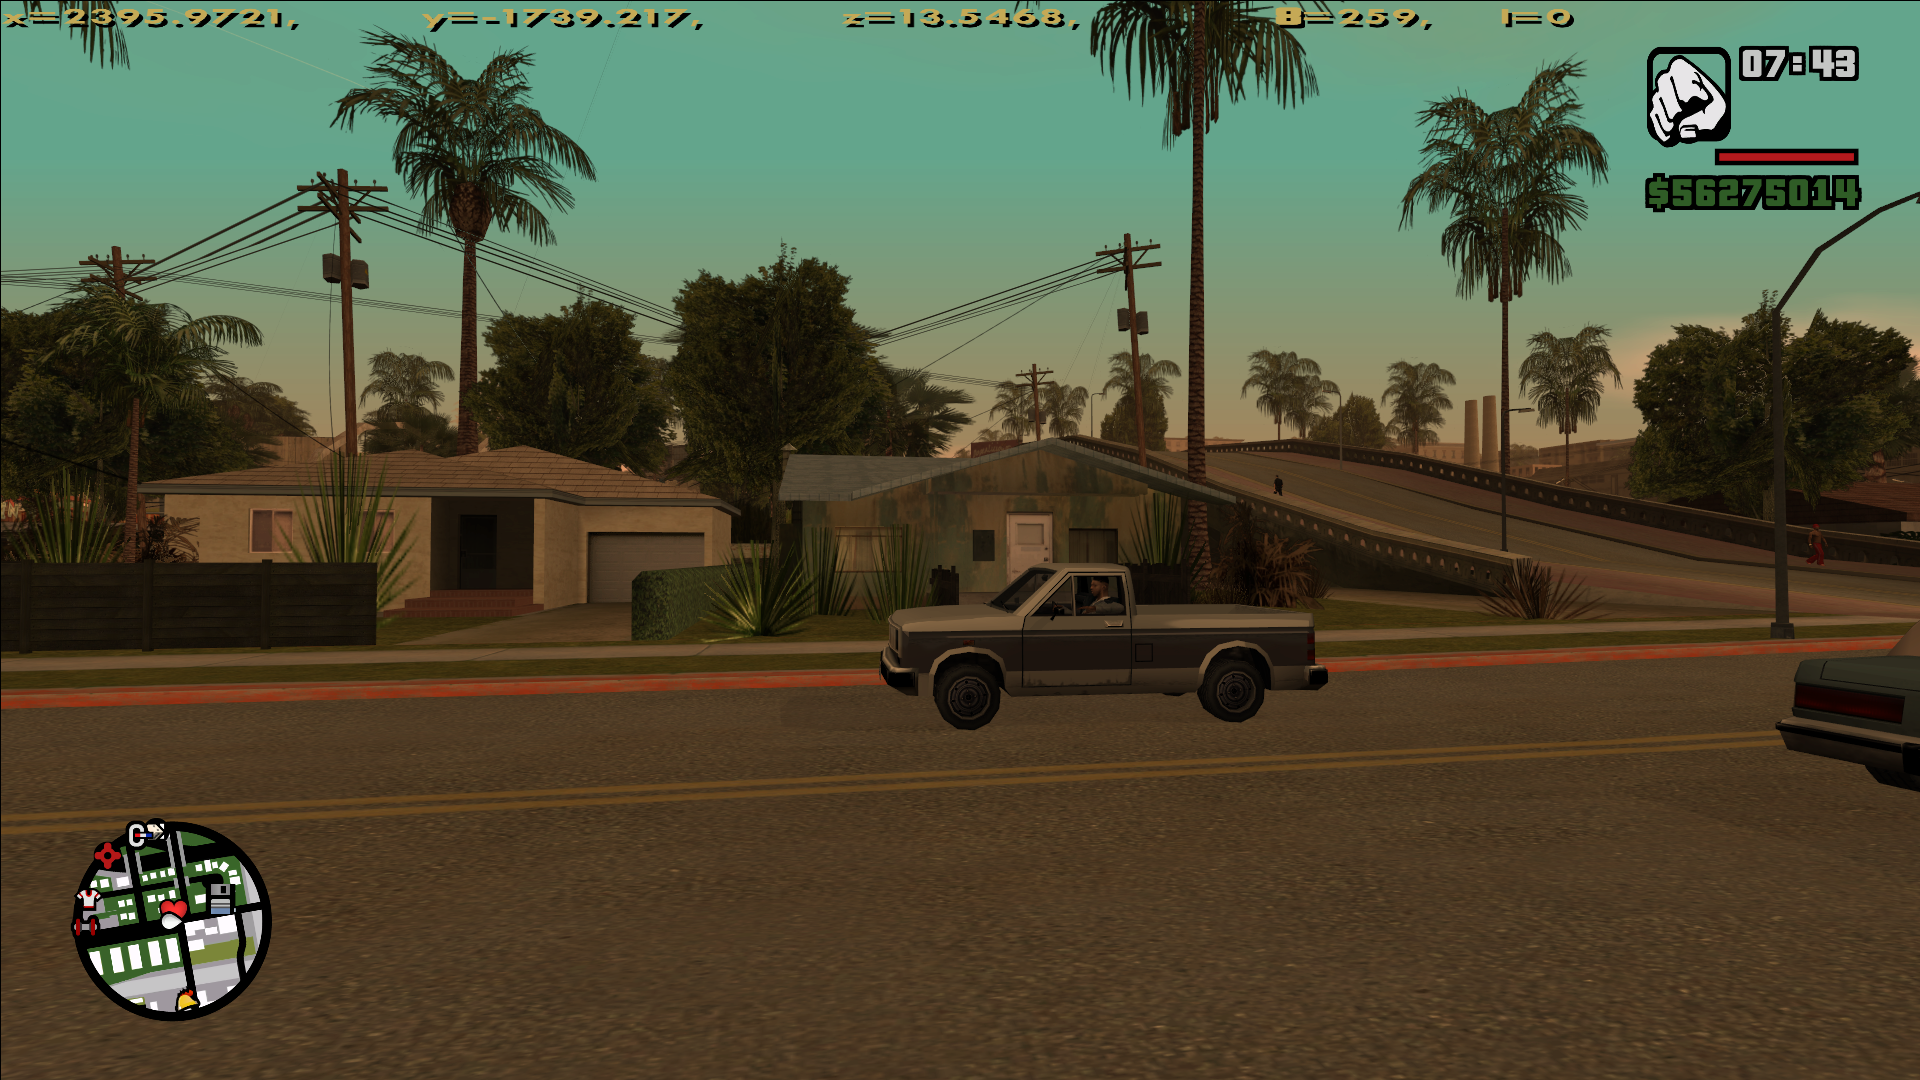
\includegraphics[width= 1\textwidth]{./0img/sinkVertex.png}
			\subcaption{Desired Location \(GF\)}
		\end{minipage}
			\hfill
		\begin{minipage}{1.0\textwidth}
			\centering
			\includesvg[width=1\textwidth]{./0img/sourceToSink}
			\subcaption{Source \(S\) to Sink \(GF\)}
		\end{minipage}
		\caption{Source and Sink In-game Location}
	\end{figure} Say we want to go from vertex \(S\) to vertex \(GF\) as illustrated from the in-game figure above and its graph. Where we need to find the shortest \(S-GF\) path. Then its shortest route will be
	\clearpage
	\begin{figure}[!h]
		\centering
		\includesvg[width=1\textwidth]{./0img/shortestRoute}
		\caption{\centering Shortest Route \\ From Vertex \(S\) to Vertex \(GF\)}
		\label{shortest_route}
	\end{figure} Observing graph figure (\ref{shortest_route}), we start at vertex \(S\) straight to through vertex \(V_{2}\) which we can see from the in-game image below.
	\clearpage
	\begin{figure}[!h]
		\centering
		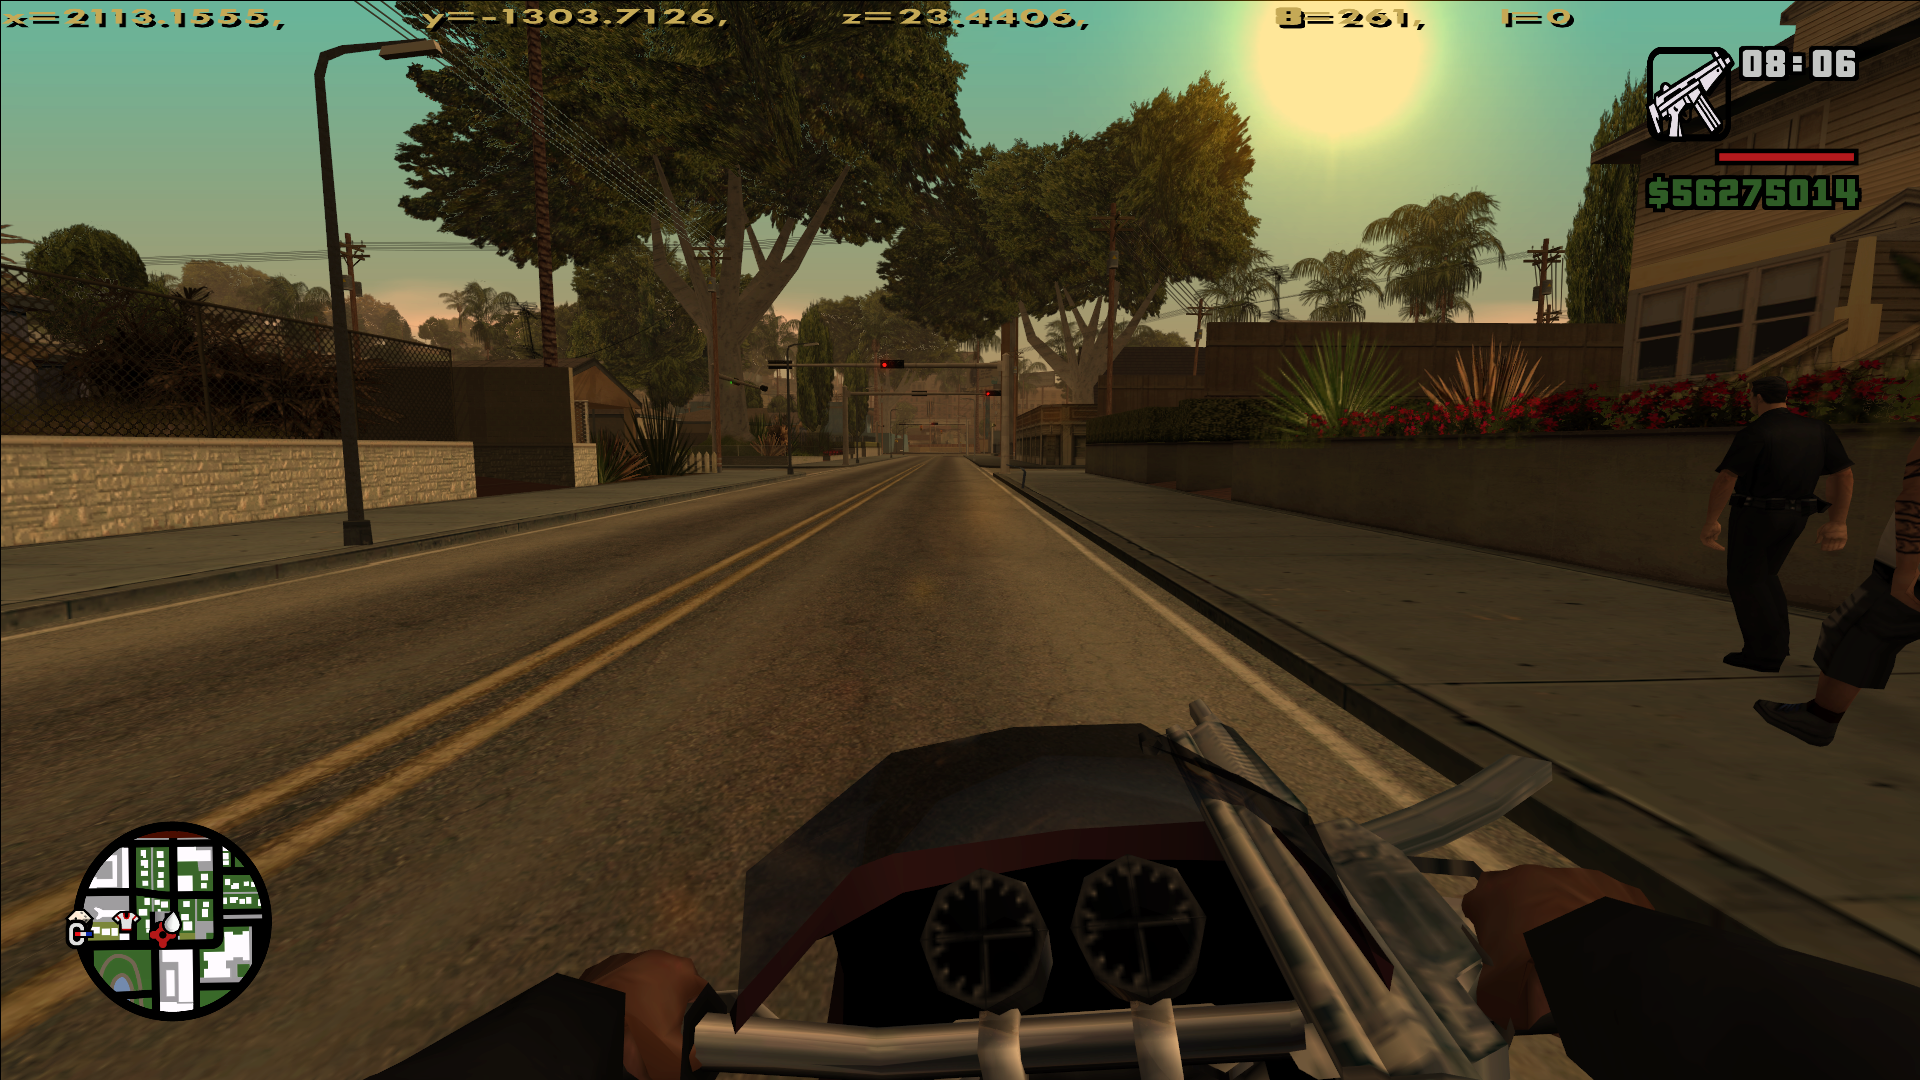
\includegraphics[width=\textwidth]{./0img/path1}
		\caption{Path \\ \(S \to V_{1} \to V_{2}\)}
	\end{figure} Then we move from \(V_{2}\) up to \(V_{6}\), then \(V_{7}\).
		\begin{figure}[!h]
		\centering
		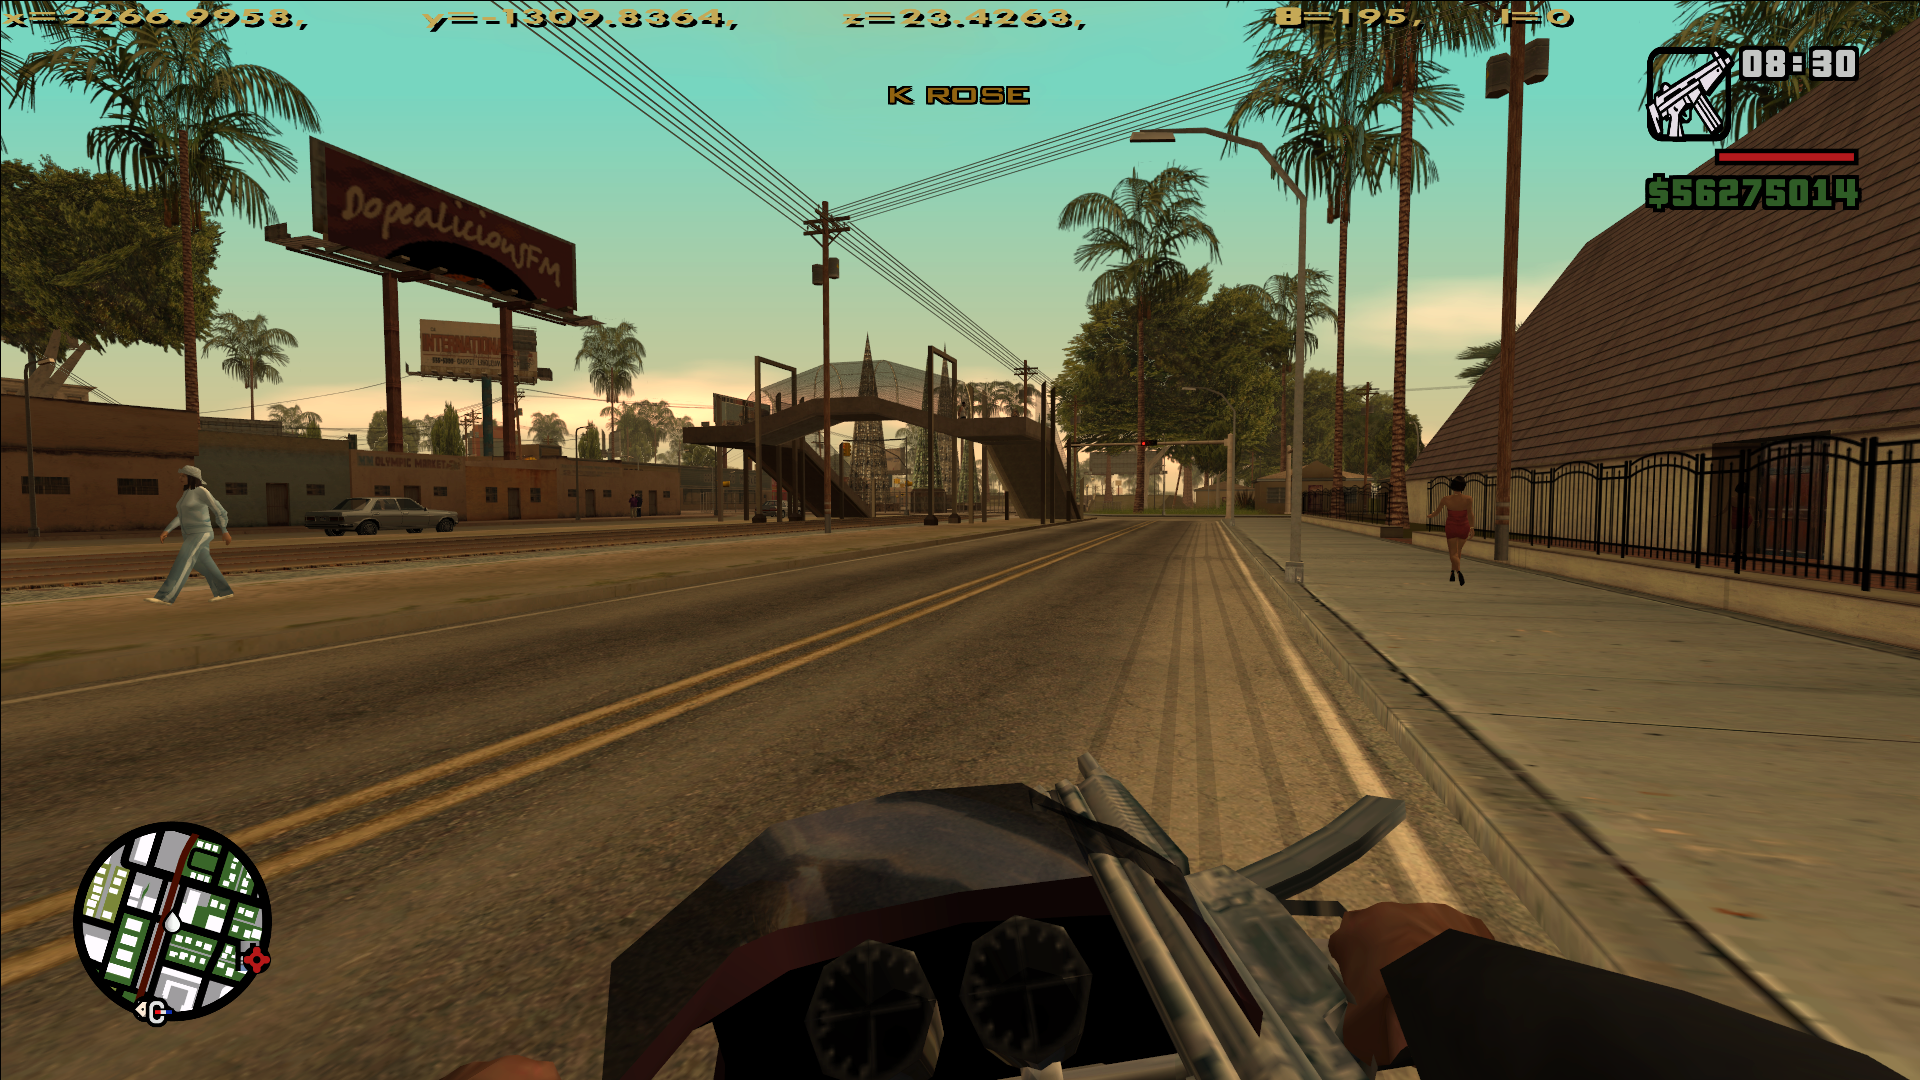
\includegraphics[width=\textwidth]{./0img/path2}
		\caption{Path \\ \(V_{2} \to V_{6} \to V_{21} \to V_{7}\)}
	\end{figure} Next, we go straight through the bridge from \(V_{7}\) until \(V_{13}\).
	From the bridge, we shall go straight ahead until \(V_18\).
	\clearpage
	\begin{figure}[!h]
		\centering
		\begin{minipage}{\textwidth}
			\centering
			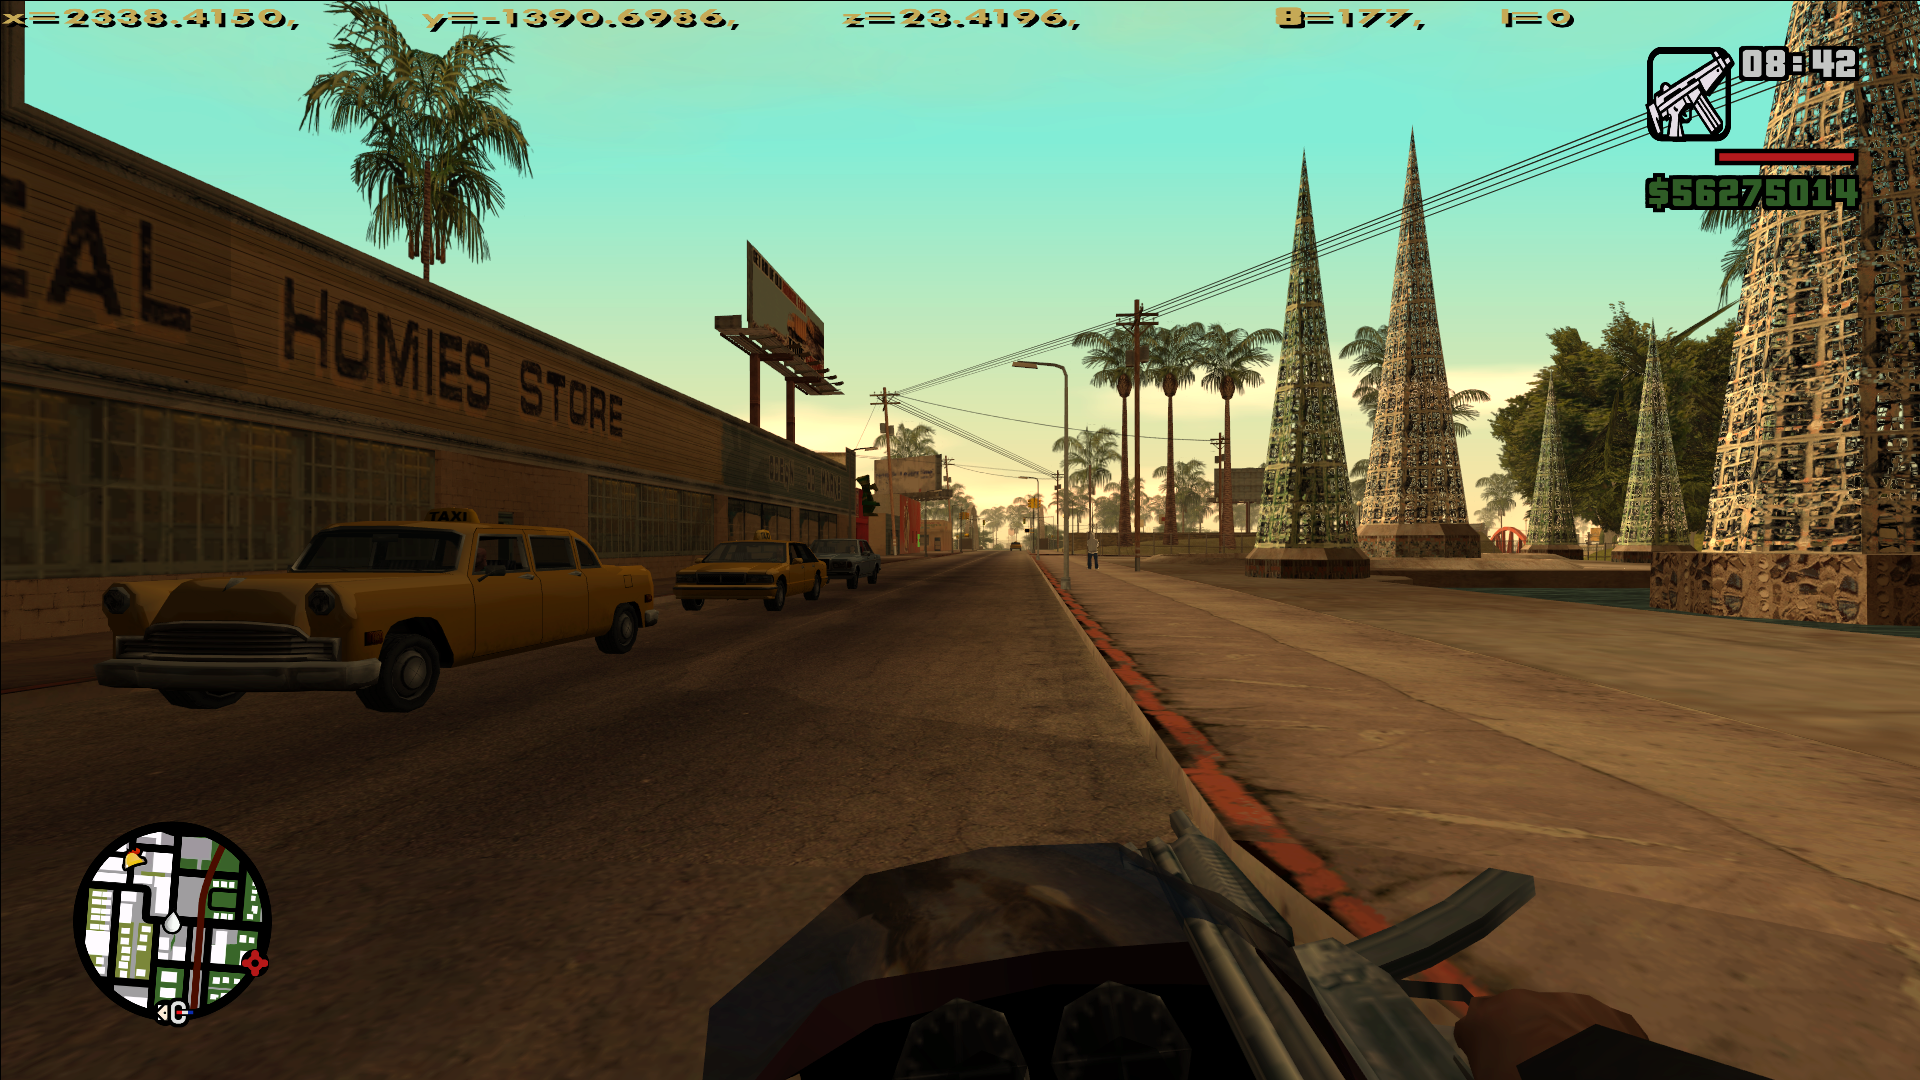
\includegraphics[width=1\textwidth]{./0img/path3.png}
			\subcaption{Path \(V_{7} \to V_{10} \to V_{24} \to V_{13}\)}
		\end{minipage}
		\hfill
		\begin{minipage}{\textwidth}
			\centering
			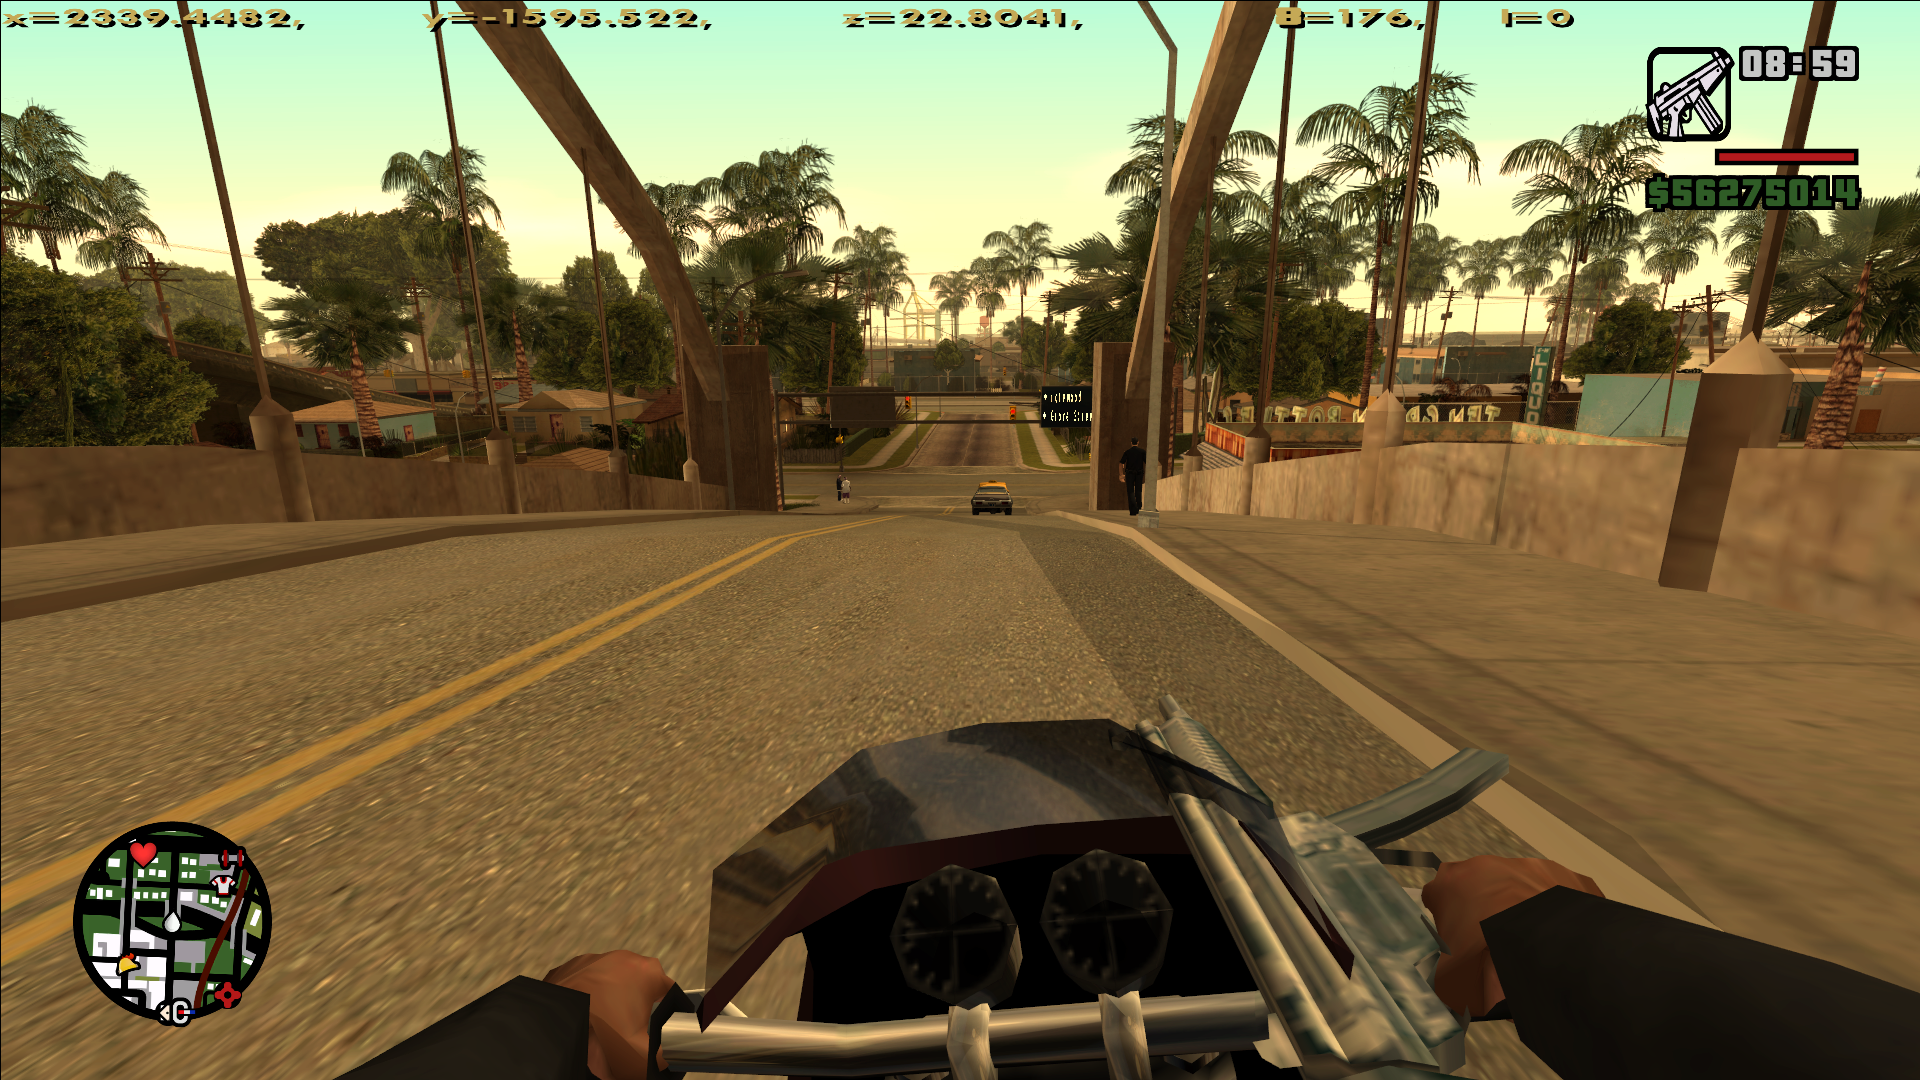
\includegraphics[width= 1\textwidth]{./0img/path4.png}
			\subcaption{Path \(V_{13} \to V_{17} \to V_{18}\)}
		\end{minipage}
		\caption{Straight through the Bridge}
	\end{figure} Finally we move from \(V_{18}\) to our final location \(GF\), where we arrived at the optimal distance to travel from the Carl's safe house \(S\) to his girlfriend's place \(GF\).
	\clearpage
	\begin{figure}[!h]
		\centering
		\begin{minipage}{\textwidth}
			\centering
			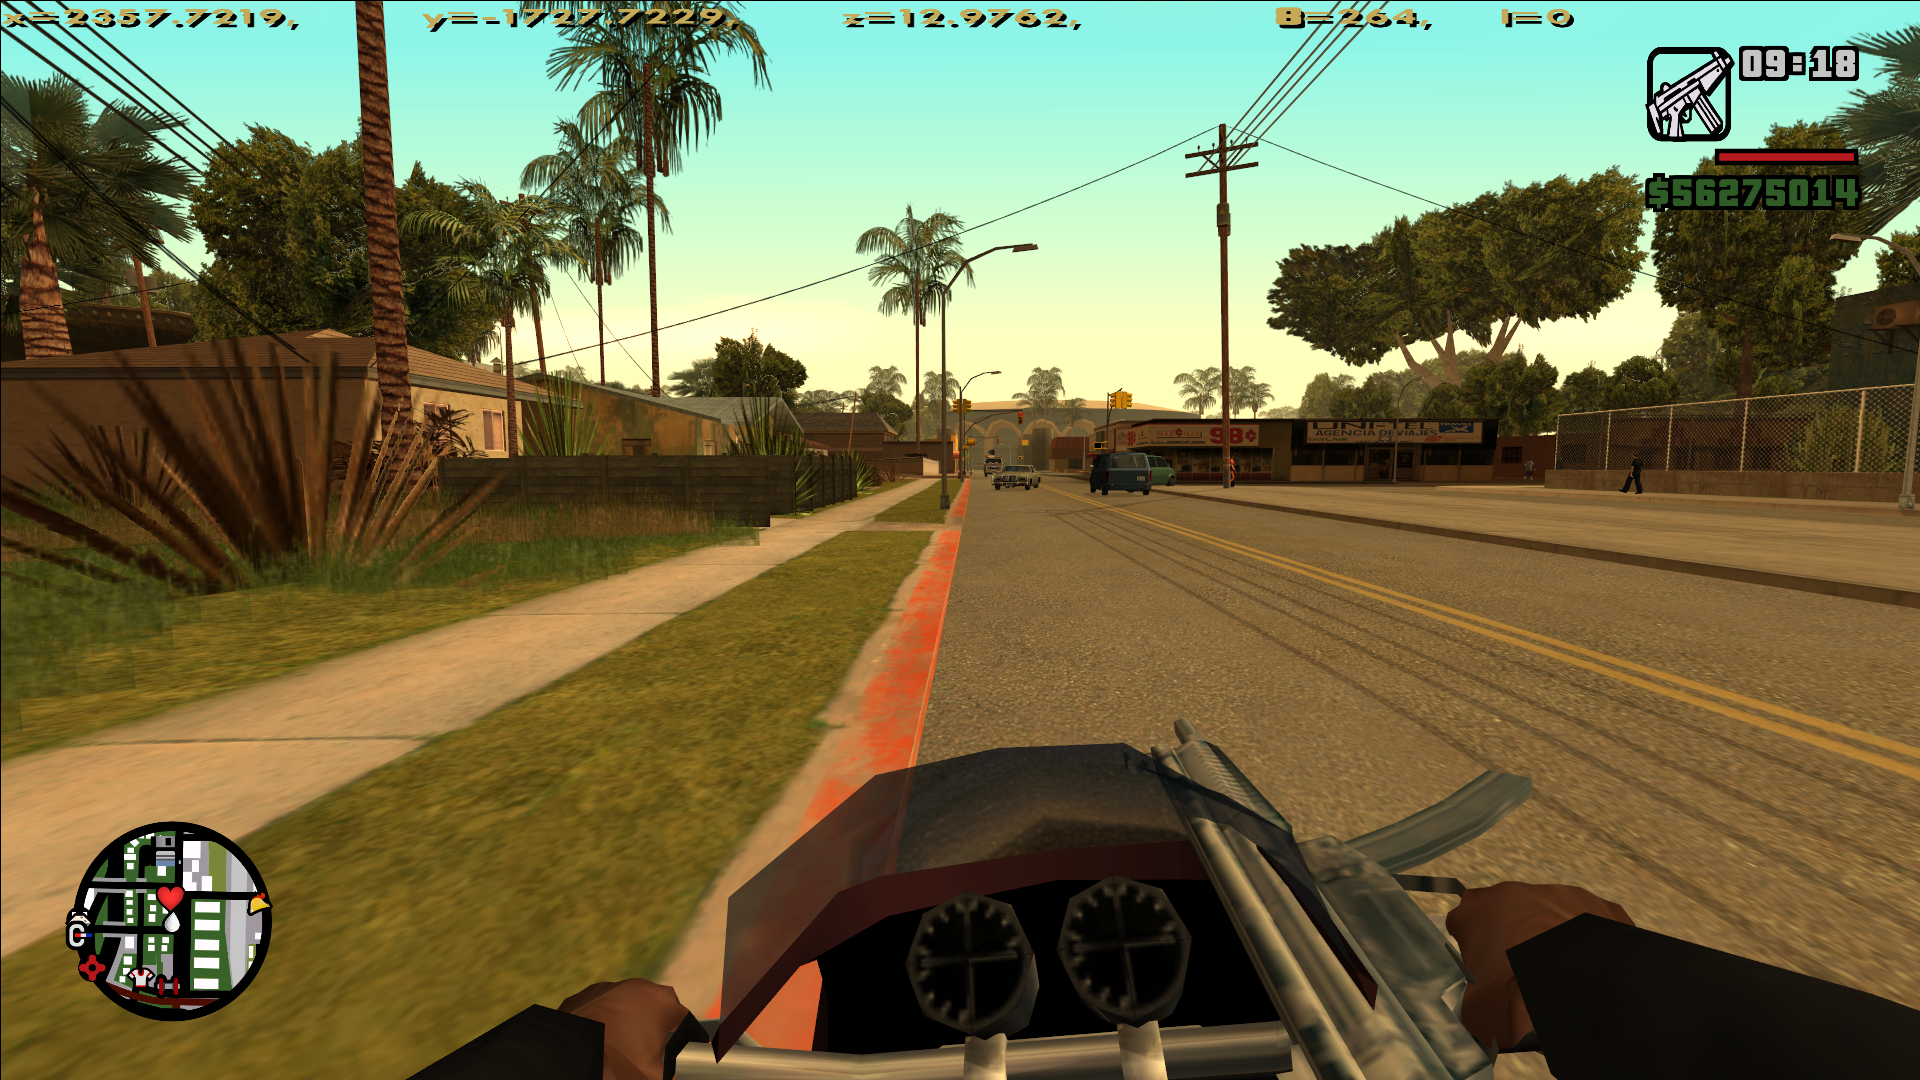
\includegraphics[width=1\textwidth]{./0img/path5.png}
			\subcaption{Path \(V_{18} \to GF\)}
		\end{minipage}
		\hfill
		\begin{minipage}{\textwidth}
			\centering
			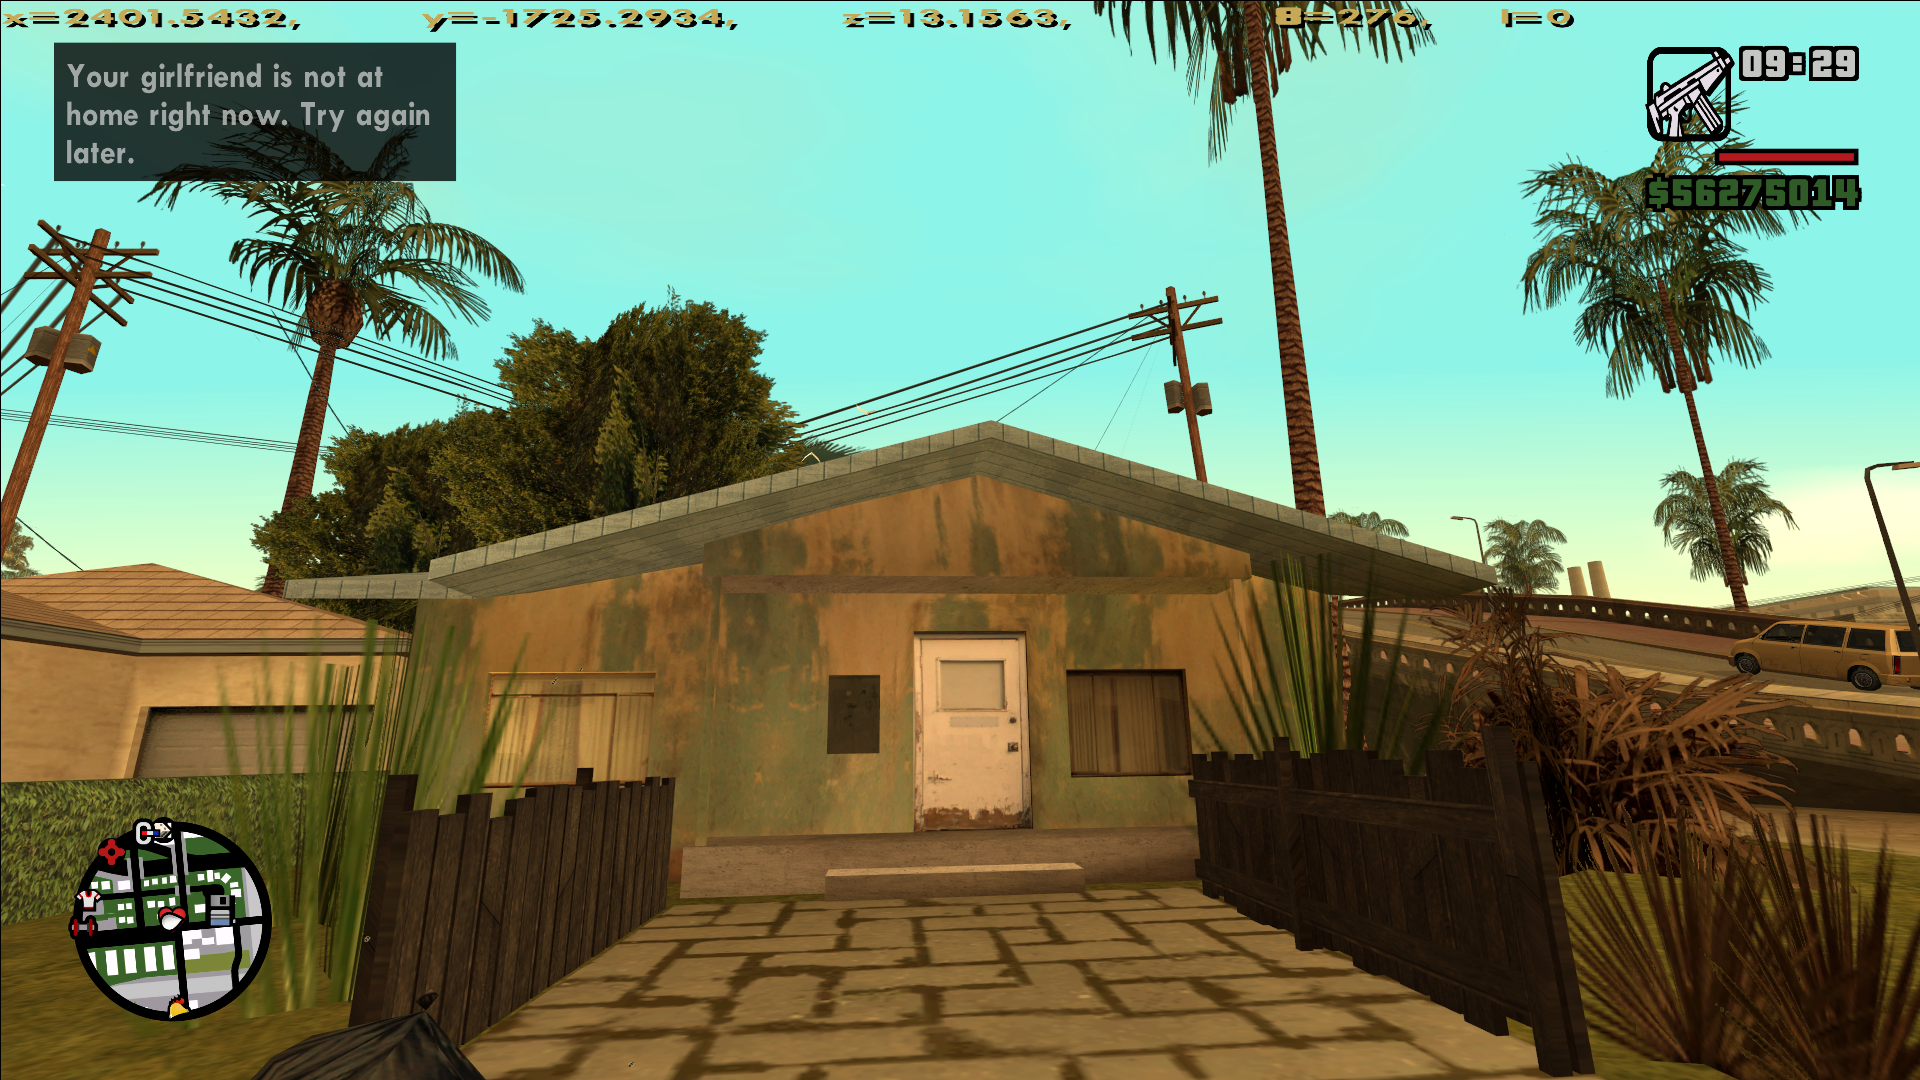
\includegraphics[width= 1\textwidth]{./0img/path6.png}
			\subcaption{Ending Position \(GF\)}
		\end{minipage}
		\caption{Final Path}
	\end{figure}
	
	\clearpage
	The table below provides as to how we utilized the shortest route algorithm.
	\begin{longtable}[c]{@{}cll|l@{}}
		\toprule
		\textbf{Vertex} &
		\textbf{\begin{tabular}[c]{@{}c@{}}Shortest \\ Distance\end{tabular}} &
		\textbf{\begin{tabular}[c]{@{}c@{}}Previous \\ Vertex\end{tabular}} &
		\multicolumn{1}{c}{\(\text{Optimal Value} = 784.21\unit{\meter}\)} \\* \midrule
		\endfirsthead
		%
		\multicolumn{4}{c}%
		{{\bfseries Table \thetable\ continued from previous page}} \\
		\endhead
		%
		\bottomrule
		\endfoot
		%
		\endlastfoot
		%
		{\color[HTML]{FF0000} S} &
		{[}0{]} &
		{[}S{]} &
		Visited = \parbox{6cm}{S, V25, V1, V26, V27, V4, V2, V5, V6, V21, V11, V7, V22, V3, V28, V8, V10, V9, V24, V13, V29, V15, V23, V16, V12, V17, V14, V20, V19, V18, GF} \\ \\
		{\color[HTML]{FF0000} V1} &
		{[}\(\infty\), 62.84{]} &
		{[}S{]} &
		Unvisited = {\color[HTML]{FE0000} \parbox{6cm}{S, V1, V2, V3, V4, V5, V6, V7, V8, V9, V10, V11, V12, V13, V14, V15, V16, V17, V18, V19, V20, V21, V22, V23, V24, V25, V26, V27, V28, V29, GF}} \\
		{\color[HTML]{FF0000} V2}  & {[}\(\infty\), 163.22{]}         & {[}V1{]}       &  \\
		{\color[HTML]{FF0000} V3}  & {[}\(\infty\), 339.6{]}          & {[}V21{]}      &  \\
		{\color[HTML]{FF0000} V4}  & {[}\(\infty\), 145.45{]}         & {[}V1{]}       &  \\
		{\color[HTML]{FF0000} V5}  & {[}\(\infty\), 192.69{]}         & {[}V4{]}       &  \\
		{\color[HTML]{FF0000} V6}  & {[}\(\infty\), 244.87{]}         & {[}V2{]}       &  \\
		{\color[HTML]{FF0000} V7}  & {[}\(\infty\), 307.05{]}         & {[}V21{]}      &  \\
		{\color[HTML]{FF0000} V8}  & {[}\(\infty\), 416.29, 406.14{]} & {[}V22, V3{]}  &  \\
		{\color[HTML]{FF0000} V9}  & {[}\(\infty\), 423.33{]}         & {[}V22{]}      &  \\
		{\color[HTML]{FF0000} V10} & {[}\(\infty\), 417.18, 407.15{]} & {[}V11, V7{]}  &  \\
		{\color[HTML]{FF0000} V11} & {[}\(\infty\), 288.4{]}          & {[}V5{]}       &  \\
		{\color[HTML]{FF0000} V12} & {[}\(\infty\), 565.3{]}          & {[}V13{]}      &  \\
		{\color[HTML]{FF0000} V13} & {[}\(\infty\), 469.29{]}         & {[}V24{]}      &  \\
		{\color[HTML]{FF0000} V14} & {[}\(\infty\), 596.66{]}         & {[}V13{]}      &  \\
		{\color[HTML]{FF0000} V15} & {[}\(\infty\), 491.9{]}          & {[}V11{]}      &  \\
		{\color[HTML]{FF0000} V16} & {[}\(\infty\), 542.57{]}         & {[}V15{]}      &  \\
		{\color[HTML]{FF0000} V17} & {[}\(\infty\), 585.92{]}         & {[}V13{]}      &  \\
		{\color[HTML]{FF0000} V18} & {[}\(\infty\), 685.01{]}         & {[}V17{]}      &  \\
		{\color[HTML]{FF0000} V19} & {[}\(\infty\), 617.78{]}         & {[}V16{]}      &  \\
		{\color[HTML]{FF0000} V20} & {[}\(\infty\), 598.07{]}         & {[}V29{]}      &  \\
		{\color[HTML]{FF0000} V21} & {[}\(\infty\), 257.97{]}         & {[}V6{]}       &  \\
		{\color[HTML]{FF0000} V22} & {[}\(\infty\), 335.77{]}         & {[}V7{]}       &  \\
		{\color[HTML]{FF0000} V23} & {[}\(\infty\), 507.43{]}         & {[}V9{]}       &  \\
		{\color[HTML]{FF0000} V24} & {[}\(\infty\), 454.42{]}         & {[}V10{]}      &  \\
		{\color[HTML]{FF0000} V25} & {[}\(\infty\), 23.62{]}          & {[}S{]}        &  \\
		{\color[HTML]{FF0000} V26} & {[}\(\infty\), 105.63{]}         & {[}V25{]}      &  \\
		{\color[HTML]{FF0000} V27} & {[}\(\infty\), 143.9{]}          & {[}V26{]}      &  \\
		{\color[HTML]{FF0000} V28} & {[}\(\infty\), 366.98{]}         & {[}V27{]}      &  \\
		{\color[HTML]{FF0000} V29} & {[}\(\infty\), 487.19{]}         & {[}V28{]}      &  \\
		{\color[HTML]{FF0000} GF}  & {[}\(\infty\), 789.64, 784.21{]} & {[}V23, V18{]} &  \\* \bottomrule
		\caption{Shortest Route Table for \(S-GF\) path}
		\label{shortest_sgf}\\
	\end{longtable}
	
	\ifx\graphTheoryPreambleLoaded
\end{document}
\fi